\chapter{How to Write Your Own Extensions and Possibly Contribute Them to MATSim}
\label{ch:extensionpoints}
% ##################################################################################################################
\hfill \textbf{Author:} Michael Zilske

\section*{Note}

Documentation for the concepts described in this chapter can be found under \url{http://matsim.org/javadoc} $\to$ main distribution, by going to the corresponding class and interface documentation entries.  These should also point to examples.

% ##################################################################################################################
\section{Introduction}
\label{sec:ownmodules-intro}
The three main elements of the \gls{matsim} cycle---execution, scoring, and \gls{replanning} (Section~\ref{sec:co-ev})---operate on what is essentially an in-memory object-oriented data base of \lstinline|Person| objects \citep{RaneyNagel2006traf-framework}.
%
These three elements are the main elements to configure \gls{matsim}:
\begin{description}\styleDescription
\item[Execution] The \gls{mobsim} can be replaced, either by an internally available alternative, or by a fully external \gls{mobsim}.
\item[Scoring] The scoring can be replaced, by possibly giving each individual agent a different recipe to compute its score.
\item[Replanning] Arbitrary implementations of type \lstinline|PlanStrategy| can be added to the \gls{replanning}; these either generate new plans from scratch or by mutating existing ones, or they select between plans.
\end{description}
%
The simulation's behavior can be further configured by using so-called \lstinline|ControlerListener|s.

The \gls{mobsim} generates a stream of \glspl{event}. These are primarily used in two places:
\begin{itemize}\styleItemize
\item The scoring uses them to track each agent's success at executing its plan, and compute the scoring value based on this.
\item \lstinline|PlanStrategy| modules use them to build approximate models of the world in which they operate. For example, the router obtains time-dependent expected link travel times from a \lstinline|TravelTime| object, which in turn listens to link enter and link exit events.
\end{itemize}
%% In consequence, each \lstinline|PlanStrategy| module can use events to obtain information about the world in which the plans of the synthetic travelers need to be improved. 
Additionally, one can write any sort of event handlers for analysis during the iterations, or after a run by evaluating the events file.

Some modules are so large that fully replacing them in order to adapt the simulation system to one's need is too much work. These are, in particular,
\begin{itemize}\styleItemize
\item the \gls{qsim}, which is the default implementation of the \lstinline|Mobsim| interface, and
\item the router.
\end{itemize}
In consequence, it is possible to add additional executable code into the execution flow of the \gls{qsim} by \lstinline|MobsimListener|s in a similar way as this is possible with the \lstinline|ControlerListener|s mentioned above.
%
The router, in contrast, is most importantly configured by replacing the definition of the generalized travel cost. 

% ##################################################################################################################
\section{Extension Points}
\label{sec:matsim-spi}
This section describes what could be called the \gls{spi} of \gls{matsim}.
Historically, the main entry-point for writing a \gls{matsim} \gls{extension} has been to literally extend (in the \gls{java} sense, i.e.\ to inherit from) the \lstinline|Controler| class. Essentially, one would override the methods calling the \gls{mobsim}, the scoring, and/or the replanning, as explained in Section~\ref{sec:ownmodules-intro}. This is now discouraged. While this pattern worked when a each member of the team was working on extending the \gls{matsim} core by a different aspect, it fails when it comes to integrating those aspects to a single product: There is nothing one can do with a \lstinline|PublicTransportControler|, an \lstinline|EmissionsControler|, a \lstinline|RoadPricingControler| and an \lstinline|OTFVisControler|, if one wants to combine them to visualize the emissions of buses on toll roads.

% =========================================================================================
\subsection{Config Group}
\label{sec:config}
The configuration of a \gls{matsimrun} is a grouped list of key-value pairs, stored in \gls{xml} format in the \gls{configfile} (see Section~\ref{sec:config}).
%Recall that it is grouped and looks, for example, like this:
%%
%\begin{lstlisting}
%<module name="qsim" >
		%<param name="flowCapacityFactor" value="0.2" />
		%<param name="storageCapacityFactor" value="0.3" />
%</module>
%
%<module name="transit" >
		%<!-- Comma-separated list of transportation modes that are handled as transit. -->
		%<param name="transitModes" value="pt" />
%
		%<!-- Input file containing the transit schedule to be simulated. -->
		%<param name="transitScheduleFile" value="network/transitSchedule.xml.gz" />
%</module>
%\end{lstlisting}
%\ah{shown earlier}

At runtime, the entire configuration is stored in an instance of \lstinline|Config|, from which instances of \lstinline|ConfigGroup| can be accessed by their name.  Config groups that are not in the main distribution need to be explicitly loaded; an approximate example is the following:
\begin{lstlisting}
MyExternalConfigGroup myConfig 
   = ConfigUtils.addOrGetModule(controler.getConfig(),
      MyExternalConfigGroup.GROUP_NAME, 
      MyExternalConfigGroup.class);
\end{lstlisting}

The author of an extension can subclass the \lstinline|ConfigGroup| class to provide named accessors for the parameters.  A possibly better way is to subclass from
%% \kaitodo{Es gibt da auch noch ein loadConfig, was AUCH die config groups ``materialisiert''.  Hm.}
%% Furthermore, there is a utility class 
\lstinline|ReflectiveConfigGroup|, which you can use if you want to define the mapping of named parameters to accessors using \gls{java} annotations.  
%% \kaitodo{See ... for an example.}

% =========================================================================================
\subsection{ObjectAttributes and Customizable}
\label{sec:objectAttributes-and-customizable}
\gls{matsim} operates on data types such as links, nodes, persons, or vehicles. Many of these data types have attributes, such as free speed (for links) or coordinates (for nodes).  Rather often, one would like additional information for certain data types, such as ``slope'' for links, or ``age'' for persons.  In order to not modify the data types every time this becomes necessary, but still allow experimentation, a helper container called \lstinline{ObjectAttributes} is available.  It essentially attaches arbitrary additional information to objects \emph{that have an \gls{id}}, by a syntax of type
\begin{lstlisting}
attribs.putAttribute( id, attribName, attribValue ) ;  
\end{lstlisting}
where \lstinline{id} is the object's \gls{id}, \lstinline{attribName} is the name (type) of the attribute to be stored (e.g.\ ``age''), and \lstinline{attribValue} is the value of the attribute (e.g.\ ``24''). 

Importantly, the package provides readers and writers for such attributes.  It is thus possible for additional code to, say, generate additional attributes by preprocessing, write them to file, and read them back for every run.  That approach is used, for example, by the Gauteng scenario (Chapter~\ref{ch:gauteng}) to pre-allocate e-tag ownership to persons.

For additional information see the \lstinline{ObjectAttributes} class under \url{http://matsim.org/javadoc} $\to$ main distribution.

Note that there is currently no simple way to similarly attach information to data types that do not have an \gls{id}.  This is, for example, the case with plans, activities, or legs, which are contained inside a data type with an \gls{id} (the person data type), but which do not possess an \gls{id} of their own and are therefore not addressable by \lstinline{ObjectAttributes}.  Some of these non-identifiable data types implement the \gls{java} interface \lstinline{Customizable}, to which additional material can be attached by a syntax of type
\begin{lstlisting}
plan.getCustomAttributes.put("myAttribName",myAttribValue) ;
\end{lstlisting}
For additional information, see the \lstinline{Customizable} interface under \url{http://matsim.org/javadoc} $\to$ main distribution.
Note that information contained in \lstinline{Customizable} is not considered standard information by \gls{matsim}.  It is not written to file when writing the corresponding container, it is in consequence not read from file, and it is undefined if it is copied when copying the data object (e.g.\ when cloning plans for the evolutionary algorithm).---This is the status quo; the \gls{matsim} team is thinking about better solutions.

% =========================================================================================
\subsection{ScenarioElement}
\label{sec:scenario-extension-point}
The object-oriented in-memory database which holds the \lstinline|Person| objects with their plan memories is accessible via the \lstinline|Population| interface. The \lstinline|Network| interface gives access to the traffic network graph, consisting of links and nodes. There is a \lstinline|TransitSchedule| interface which represents the public transit schedule. Your own modeling tasks may need an additional data container like these. We call them scenario elements. The freight carrier population of the freight \gls{extension} described in Section~\ref{sec:carriers} is a typical example. 

\lstinline|Scenario| is the interface which ties all scenario elements together. You can add your own named scenario element to the \lstinline|Scenario| at startup, for example in a \lstinline|StartupListener|. All standard scenario elements are populated from \gls{xml} files at startup, but your own scenario elements could just as well be interfaces to an external relational database.

% =========================================================================================
\subsection{ControlerListener: Handling Controler Events}
\label{sec:controlerListener-extension-point}
% \label{sec:controlerextension} \ah{double label working?}
\lstinline|Controler| remains the main user-facing class of \gls{matsim}, but please do not subclass it. 
Rather, use its setter methods to plug in your own code. 

\lstinline|ControlerListeners| are called at the transitions of the \gls{matsim} loop (Figure~\ref{fig:controlerevents}), where so-called \lstinline|ControlerEvent|s are fed to the listeners. 
% ------------
\createfigure%
{Controler events}%
{Controler events}%
{\label{fig:controlerevents}}%
{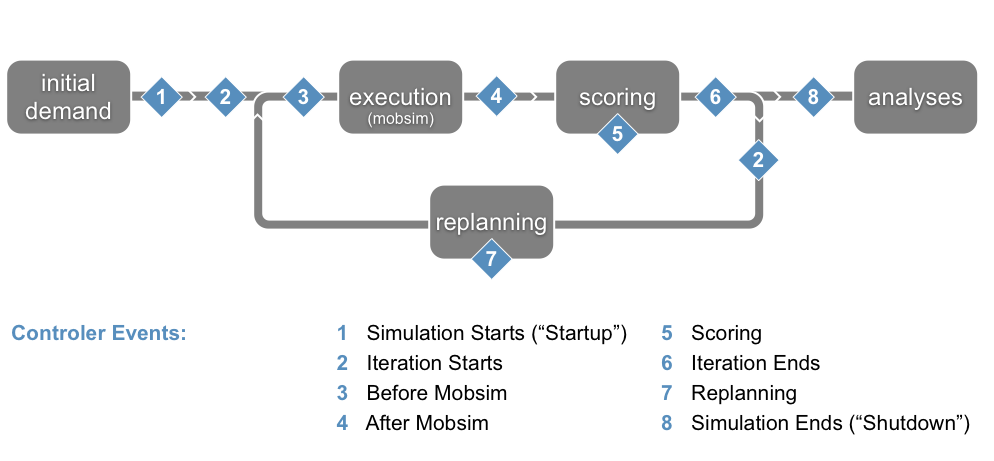
\includegraphics[width=0.99\textwidth, angle=0]{extending/figures/controler_listeners.png}}%
{}
% ------------

The following \lstinline|ControlerListeners| are currently available:
\lstinline|StartupListener|,
\lstinline|IterationStartsListener|,
\lstinline|BeforeMobsimListener|,
\lstinline|AfterMobsimListener|,
\lstinline|ScoringListener|,
\lstinline|IterationEndsListener|,
\lstinline|ReplanningListener|, and
\lstinline|ShutdownListener|.  An up-to-date list can be obtained from \url{http://matsim.org/javadoc} $\to$ main distribution $\to$ \lstinline{ControlerListener} interface.

A sample listener might look as follows.
\begin{lstlisting}
public class MyControlerListener implements StartupListener { 
   @Override 
   public void notifyStartup(StartupEvent event) { 
      ...
   }
} 
\end{lstlisting}

\lstinline|ControlerListeners| are called in undefined order, meaning that \lstinline|AControlerListener| may only rely on the computation of \lstinline|BControlerListener| if \lstinline|BControlerListener| makes that computation in an earlier transition. For instance, if \lstinline|BControlerListener| is a \lstinline|StartupListener| and loads data into a \lstinline|Map| on start-up, \lstinline|AControlerListener| can be an \lstinline|IterationStartsListener| and use that \lstinline|Map|. But do not write two \lstinline|IterationStartsListeners| where the first puts some data into a \lstinline|Map| and the second expects to find it there---they may be called in any order.

%% \kaitodo{Bild?!}
%% \ah{Habe das noch ein wenig ergänzt, mit Hilfe von \url{http://www.matsim.org/node/602}. Please check.}
%% \kaitodo{check}


% =========================================================================================
\subsection{Mobsim Events}
\label{sec:events-extension-point}
The \gls{mobsim} moves the agents around in the virtual world according to their plans and within the bounds of the simulated reality. 
It documents their moves by producing a stream of \glspl{event}. 
Events are small pieces of information describing the action of an object at a specific time. Examples of such events are (see also Figure~\ref{fig:events-overview}):
\begin{itemize}\styleItemize
\item An agent finishes an activity
\item An agent starts a trip
\item A vehicle enters a road segment
\item A vehicle leaves a road segment
\item An agent boards a public transport vehicle
\item An agent arrives at a location
\item An agent starts an activity
\end{itemize}
%
%\kai{Hier gibt es ein nettes Bild auf drupal; sollten wir noch hinzunehmen.}
% ah{added}
% ------------
\createfigure%
{Mobsim events}%
{Mobsim events} % \ah{I made an non-inline todo beacuse of compilation problems}
{\label{fig:events-overview}}%
{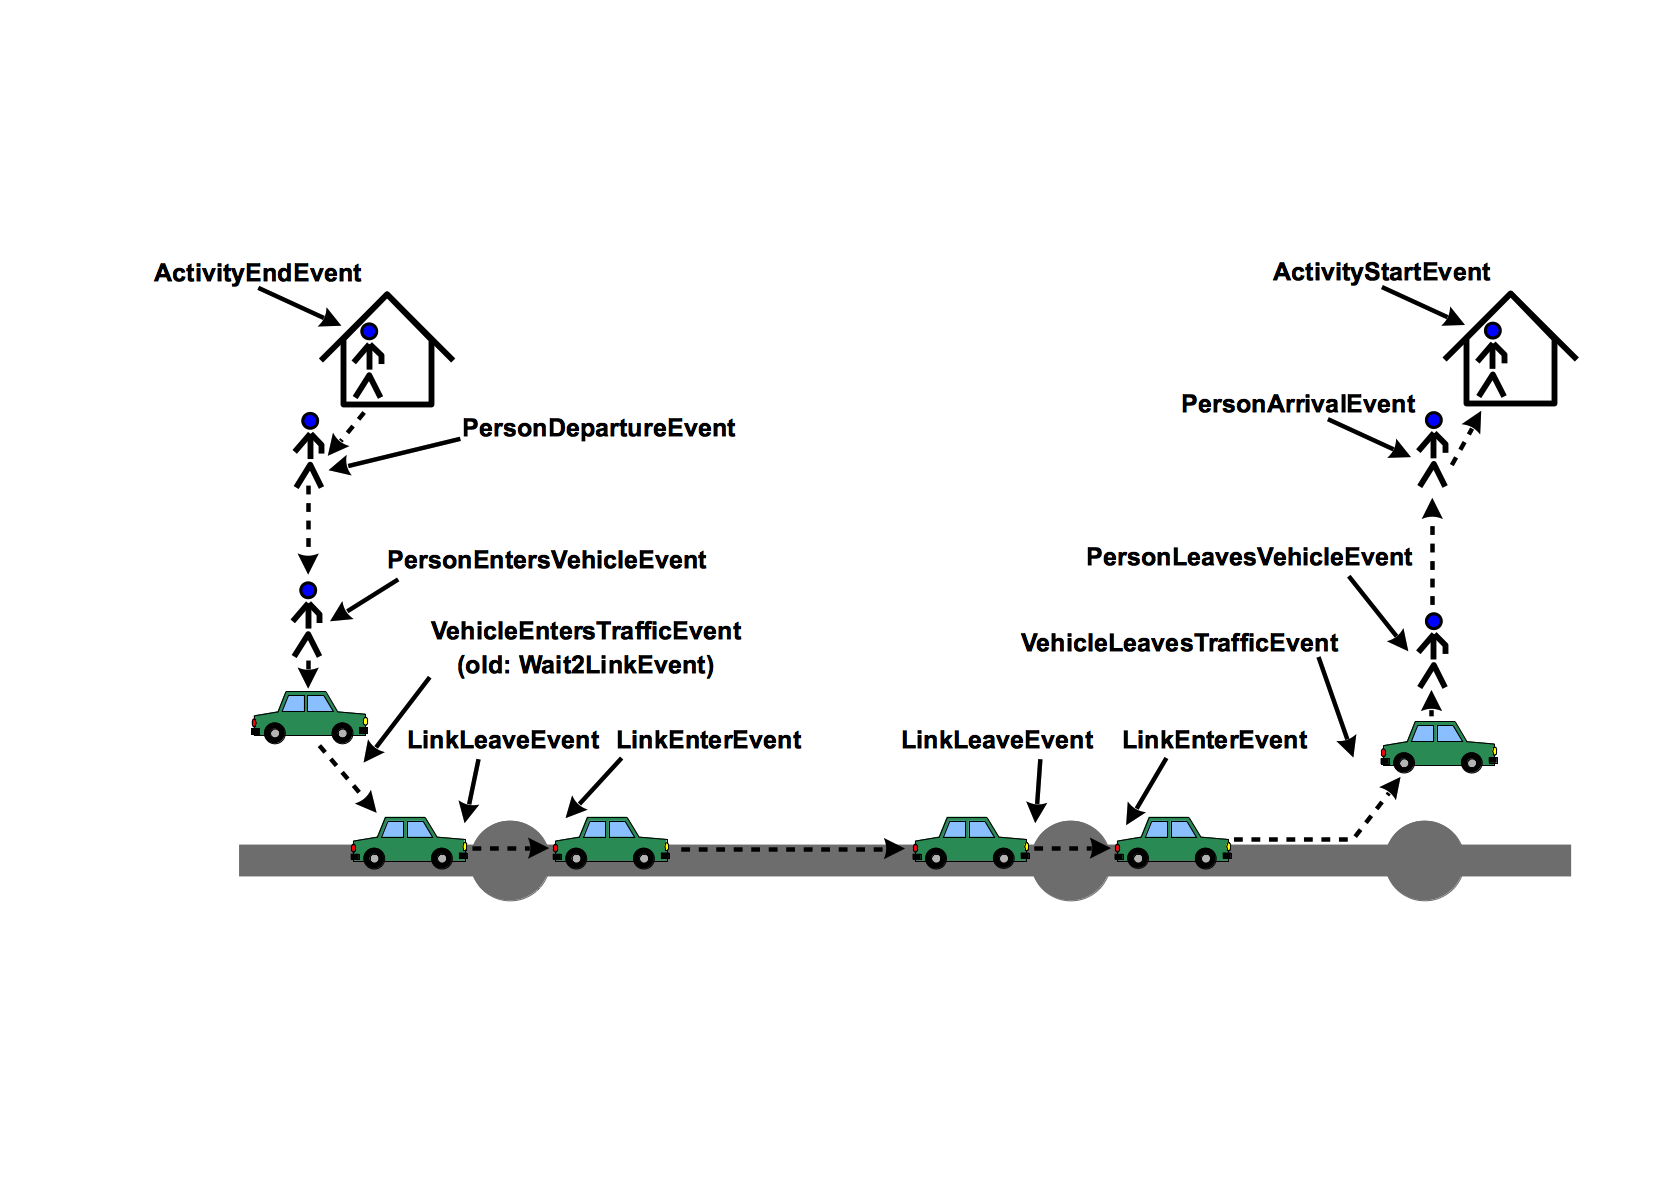
\includegraphics[width=0.6\textwidth, angle=0]{extending/figures/Events.png}}%
{}
% ------------
%
Each event has a timestamp, a type, and additional attributes required to describe the action like a vehicle id, a link id, an activity type or other data. In theory, it should be possible to replay the \gls{mobsim} just by the information stored in the events. While a \gls{plan} describes an agent's intention, the stream of events describes how the simulated day actually was.

As the events are so basic, the number of events generated by a \gls{mobsim} can easily reach a million or more, with large simulations even generating more than a billion events. But as the events describe all the details from the execution of the plans, it is possible to extract essentially any kind of aggregated data one is interested in. Practically all analyses of \gls{matsim} simulations make use of events to calculate some data. Examples of such analyses are the average duration of an activity, average trip duration or distance, mode shares per time window, number of passengers in specific transit lines and many more.

The scoring of the executed plans makes use of events to find out how much time agents spend 
% kann man vielleicht auch ``spent'' (= Vergangenheit) schreiben, aber mir erscheint Gegewart plausibler.  kai, sep'15
at activities or for traveling. Some \gls{replanning} modules might make use of \glspl{event} as well: The router for example can use the information contained in events to figure out which links are jammed at certain times and route agents around that jam when creating new plans.

% -----------------------------------------------------------------------------
\subsubsection{Handling Mobsim Events}
\gls{matsim} extensions can watch the \gls{mobsim} by interpreting the stream of \glspl{event}. This is done by implementing the \lstinline|EventHandler| interface and registering the implementation with the framework. The lifecycle of an \lstinline|EventHandler| can be chosen by the developer. Normally, an \lstinline|EventHandler| lives as long as the simulation run.
It is notified before the beginning of each new iteration so that its state can be reset to listen to a new iteration. This pattern can be used to collect information over all iterations. But if the purpose of an \lstinline|EventHandler| is to make a calculation based on one single iteration, it may be more natural to create a new \lstinline|EventHandler| instance for each iteration, query it for its result and discard it after the iteration finishes. This can be done in a \lstinline|ControlerListener|.

% -----------------------------------------------------------------------------
\subsubsection{Producing Events}
One can extend the \gls{matsim} event model by extending the \lstinline|Event| class to define own event types. \Glspl{event} can be produced from all places in the code which are executed during the running \gls{mobsim}, and in particular from other \lstinline|EventHandler| instances. Assume for example you want to analyze left-turns. A good starting point would be to specify a \lstinline|LeftTurnEvent| class, and produce an instance of this class whenever a vehicle does a left-turn. You may do this from a class which is a \lstinline|LinkLeaveEventHandler| as well as a \lstinline|LinkEnterEventHandler|. 
A \lstinline|LinkLeaveEvent| is produced every time a vehicle leaves a road segment, and a \lstinline|LinkEnterEvent| is produced when it enters the next road segment. Pairing each \lstinline|LinkLeaveEvent| with the next \lstinline|LinkEnterEvent| for the same vehicle gives a model for a vehicle crossing a node. At this point, your code would look at the road network model to determine if this was a left-turn, and if so, produce a \lstinline|LeftTurnEvent|.
    
To produce a custom \gls{event} which is not triggered by another \gls{event}, you can implement the \lstinline|MobsimListener| interface. A \lstinline|MobsimListener| is called in each simulation timestep.
For example, if you wanted to include a model of weather conditions into the simulation, you could use this extension point to decide in every time step if it should start or stop raining on a certain road segment, and produce custom events for this. You would then calculate rain exposure per agent by adding an \lstinline|EventHandler| which handles \lstinline|LinkEnterEvent|, \lstinline|LinkLeaveEvent| and your custom rain events. 

Note that \lstinline|EventHandler| and \lstinline|MobsimListener| instances may be run in parallel by the \gls{framework}. It is generally not safe to share state between them. 
The \gls{framework} guarantees that 
the methods of an \lstinline|EventHandler| instance are called sequentially, but two different instances may run on different threads of execution. Access to shared data must be synchronized externally. Whenever possible, different \lstinline|EventHandler| instances should only communicate through events.

% =========================================================================================
\subsection{TripRouter}
\label{sec:router-extension-point}
A \lstinline{TripRouter} is a service object providing methods to generate \emph{trips} between locations, given a (main) mode, a departure time and a \lstinline{Person}. A trip is a sequence of plan elements representing a movement. It typically consists of a single \glspl{leg} (\lstinline{Leg} objects), or of a sequence of \glspl{leg} with ``\emph{stage activities}'' in between. For instance, public transport trips contain \lstinline{pt interaction} activities, representing changes of vehicles in public transport trips.

% ----------------------------------------------------------------
\subsubsection{Using the Router}
A \lstinline{TripRouter} instance provides a few methods to work with trips, namely
\begin{itemize}\styleItemize
	\item Compute a route for a given mode and \gls{od} pair, for a \lstinline{Person} with a specific departure time
	\item Identify the \emph{main mode} of a trip. For instance, a trip composed of several \emph{walk} and \emph{pt} \glspl{leg} should be identified as a public transport trip.
	\item Identify which activities are \emph{stage activities}, and, by extension, identify the trips in the plan: A trip is the longest sequence of consecutive \lstinline{Leg}s and \emph{stage activities}
\end{itemize}

Please check the documentation of the \lstinline{TripRouter} class (see~\url{http://matsim.org/javadoc} $\to$ main distribution) for more details and pointers to examples.

% ----------------------------------------------------------------
\subsubsection{Configuring the Router}
The \lstinline{TripRouter} computes routes by means of \lstinline{RoutingModule} instances, one of which is associated with each mode. A \lstinline{RoutingModule} defines the way a trip is computed,
and is able to identify the \emph{stage activities} it generates.

The association between modes and \lstinline{RoutingModule} instances is configurable. You can even provide you own \lstinline{RoutingModule} implementations. Do this if your use-case requires custom routing logic, for instance if you want to implement your own complex travel mode.

Please check the documentation of the \lstinline{TripRouter} class  (see~\url{http://matsim.org/javadoc} $\to$ main distribution) for more details and pointers to examples.

% =========================================================================================
\subsection{Mobsim}
\label{sec:mobsim-extension-point}
Besides adding \lstinline|MobsimListener| implementations to enrich the standard \gls{mobsim}, it is also possible to replace the entire \gls{mobsim} by a custom implementation. A \gls{mobsim} is basically
a \lstinline|Runnable| which is supposed to take a \gls{scenario} and produce a stream of \glspl{event}. This allows you to use the co-evolutionary framework of \gls{matsim} while replacing the traffic model itself. 

Your implementation need not be written in \gls{java}. The \gls{framework} includes a helper class to call an arbitrary executable which is then expected to write its \gls{event} stream into a file. 
%
This pattern has been used successfully many times, see, \eg Section~\ref{sec:deqsim}, or the \gls{cuda} implementation of the \gls{mobsim} by \citet{Strippgen_PhDThesis_2009}.  Note that we have found consistently that an external \gls{mobsim} does \emph{not} help with computing speed: Whatever is gained in the \gls{mobsim} itself is more than lost again by the necessary data transfer between \gls{matsim} and the external \gls{mobsim}.  As of now, we cannot yet say if newer data exchange techniques, such as Google Protocol Buffers, may change the situation.  Until then, the external interface should rather be seen as the option to inject a different, possibly more realistic, \gls{mobsim} into \gls{matsim}.

% =========================================================================================
\subsection{PlanStrategy}
\label{sec:replanning-extension-point}
Replanning in \gls{matsim} is specified by defining a set of weighted strategies. In each iteration, each agent makes a draw from this set and executes the selected strategy. The strategy specifies how the agent changes its behavior. Most generally, it is an operation on the plan memory of an agent: It adds and/or removes plans, and it marks one of these plans as selected.

Strategies are implementations of the \lstinline|PlanStrategy| interface. The two most common cases are:
\begin{itemize}\styleItemize
\item Pick one plan from memory according to a specified choice algorithm.
\item Pick one plan from memory at random, copy it, mutate it in some specific aspect, add the mutated plan to the plan memory, and mark this new plan as selected.
\end{itemize}

The framework provides a helper class which can be used to implement both of these strategy templates. The helper class delegates to an implementation of \lstinline|PlanSelector|, which selects a plan from memory, and to zero, one or more implementations of \lstinline|PlanStrategyModule|, which mutate a copy of the selected plan.

The maximum size of the plan memory per agent is a configurable parameter of \gls{matsim}. Independent of what the selected \lstinline|PlanStrategy| does, the framework will remove plans in excess of the maximum from the plan memory. The algorithm by which this is done is another implementation of \lstinline|PlanSelector| and can be configured. 

The four most commonly used strategies shipped with \gls{matsim} are:
\begin{itemize}\styleItemize
\item Select from the existing plans at random, which are weighted by their current score.
\item Mutate a random existing plan by re-routing all trips.
\item Mutate a random existing plan by randomly shifting all activity end times backwards or forwards.
% and re-routing all trips.
% The standard time allocation mutator does NOT re-route.  Which makes sense (I think). kai, sep'15
\item Mutate a random existing plan by changing the mode of transport and re-routing one or more trips or tours.
\end{itemize}

Routes are computed based on the traffic conditions of the previous iteration, which are measured by means of an \lstinline|EventHandler|. Using the same pattern, your own \lstinline|PlanStrategy| can use any data which can be computed from the mobility simulation. The source code of the standard \lstinline|PlanStrategy| implementations can be used as a starting point for implementing custom behavior.

Re-routing as a building block of many \gls{replanning} strategies is a complex operation by itself. It can even be recursive: For example, finding a public transport route may consist of selecting access and egress stations as sub-destination, finding a scheduled connection between them, and finding pedestrian routes between the activity locations and the stations. With the \lstinline|TripRouter| interface, the framework includes high-level support for assembling complex modes of transport from building blocks provided by other modules or the core. 
  
% =========================================================================================
\subsection{Scoring}
\label{sec:scoring-extension-point}
% By default, MATSim uses the so-called Charypar-Nagel utility formulation to score plans. Its parameters are configurable.
The parameters of the default \gls{matsim} scoring function (Chapter~\ref{ch:scoring}) are configurable. The code, which maps a stream of \gls{mobsim} \glspl{event} to a \gls{score} for each agent is placed behind a factory interface and replaceable. However, replacing it means replacing the entire utility formulation. There is currently no mechanism for composing a utility formulation from contributions by different modules. For instance, a module which simulates weather conditions would probably calculate penalties for pedestrians walking in heavy rain, and the Cadyts (Section~\ref{ch:cadyts}) calibration scheme already uses utility offsets in its formulation. A modeler who wishes to compose a scoring function from the Charypar-Nagel utility, the rain penalty and the calibration offset needs to do this manually, in code, accessing the code of all three modules contributing to the score and (for instance) summing up their contributions. As of the writing of this chapter, this makes scoring in a way the least modular part of \gls{matsim}: It has to be re-defined, in code, for every combination of \glspl{module} which contribute to the utility.

Keep in mind that \gls{scoring} and \gls{replanning} are not inherently coupled or automatically consistent with each other. Consider a scoring function which penalizes left-turns. This is straight-forward to program: You would iterate over every route an agent has taken. Looking at the \lstinline|Network|, you would calculate for each change of links if you consider it a left-turn, and if so, add a (negative) penalty to the score. However, this would not by itself lead to a solution where routes are distributed according to this scoring function. The reason is that the default \gls{replanning} only proposes fastest routes, in other words, least-cost paths with respect to travel time. By default, the plan memory of an agent will only ever contain routes which have in one iteration been a fastest route. The behavior of the router is, in this case, inconsistent with the utility formulation.
   
% ##################################################################################################################

% Local Variables:
% mode: latex
% mode: reftex
% mode: visual-line
% TeX-master: "../main"
% comment-padding: 1
% fill-column: 9999
% End: 
